\documentclass[a4paper,12pt]{article} 

\usepackage{ctex} % 使用ctex包支持中文
\usepackage{tikz}
\usepackage{pgf}
\usepackage{amsmath}
\usepackage{color}

\usetikzlibrary {arrows.meta, automata, positioning}

\setlength{\parindent}{0pt}
\begin{document}
\section{给定正则表达式$b(a|b)^*ab$}
\subsection{用Thompson算法构造出相应的NFA\textcolor{red}{(15分)}}


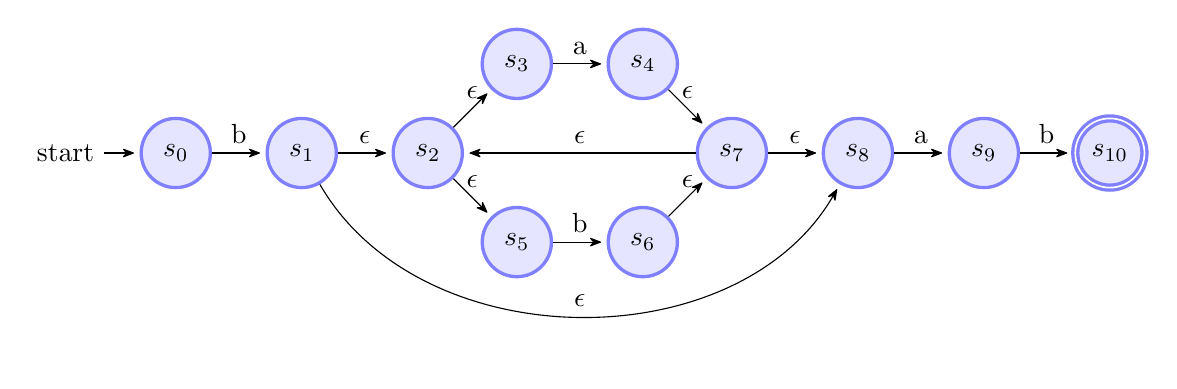
\begin{tikzpicture}[shorten >=2pt,
    node distance=1.6cm,
    on grid,
    >={Stealth[round]},
    bend angle=60,
    every state/.style={draw=blue!50,very thick,fill=blue!10}]

    \node[state,initial]  (s_0)                      {$s_0$};

    \node[state]          (s_1) [right=of s_0] {$s_1$};
    \node[state]          (s_2) [right=of s_1] {$s_2$};
    \node[state]          (s_3) [above right=of s_2] {$s_3$};
    \node[state]          (s_4) [right=of s_3] {$s_4$};
    \node[state]          (s_5) [below right=of s_2] {$s_5$};
    \node[state]          (s_6) [right=of s_5] {$s_6$};
    \node[state]          (s_7) [below right=of s_4] {$s_7$};
    \node[state]          (s_8) [right=of s_7] {$s_8$};
    \node[state]          (s_9) [right=of s_8] {$s_9$};
    \node[state,accepting]          (s_10) [right=of s_9] {$s_{10}$};

    \path[->]
    (s_0) edge              node [above]  {b} (s_1)
    (s_1) edge              node [above]  {$\epsilon$} (s_2)
    (s_1) edge [bend right]      node [above]  {$\epsilon$} (s_8)
    (s_2) edge              node [above]  {$\epsilon$} (s_3)
    (s_2) edge              node [above]  {$\epsilon$} (s_5)
    (s_3) edge              node [above]  {a} (s_4)
    (s_5) edge              node [above]  {b} (s_6)
    (s_4) edge              node [above]  {$\epsilon$} (s_7)
    (s_6) edge              node [above]  {$\epsilon$} (s_7)
    (s_7) edge              node [above]  {$\epsilon$} (s_8)
    (s_7) edge              node [above]  {$\epsilon$} (s_2)
    (s_8) edge              node [above]  {a} (s_9)
    (s_9) edge              node [above]  {b} (s_10);
\end{tikzpicture}


\subsection{用子集构造法将NFA转换为DFA,写出状态转换表\textcolor{red}{(10分)},并画出相应的DFA状态图\textcolor{red}{(10分)}}


\begin{table}[ht]
    \begin{center}
        \begin{tabular}{c|c|c|c}
            \textbf{新状态} & \textbf{NFA状态集合}                     & \textbf{a}                          & \textbf{b}                           \\
            \hline
            $q_0$        & $\{s_0\}$                            &                                     & $\{s_1, s_2, s_3, s_5, s_8\}$        \\
            \hline
            $q_1$        & $\{s_1, s_2, s_3, s_5, s_8\}$        & $\{s_2, s_3,s_4,s_5,s_7,s_8,s_9\} $ & $\{s_2,s_3,s_5,s_6,s_7,s_8\}$        \\
            \hline
            $q_2$        & $\{s_2, s_3,s_4,s_5,s_7,s_8,s_9\}$   & $\{s_2, s_3,s_4,s_5,s_7,s_8,s_9\}$  & $\{s_2,s_3,s_5,s_6,s_7,s_8,s_{10}\}$ \\
            \hline
            $q_3$        & $\{s_2,s_3,s_5,s_6,s_7,s_8\}$        & $\{s_2, s_3,s_4,s_5,s_7,s_8,s_9\}$  & $\{s_2,s_3,s_5,s_6,s_7,s_8\}$        \\
            \hline
            $q_4$        & $\{s_2,s_3,s_5,s_6,s_7,s_8,s_{10}\}$ & $\{s_2, s_3,s_4,s_5,s_7,s_8,s_9\}$  & $\{s_2,s_3,s_5,s_6,s_7,s_8\}$        \\
            \hline
        \end{tabular}
        \caption{状态转换表}
    \end{center}
\end{table}
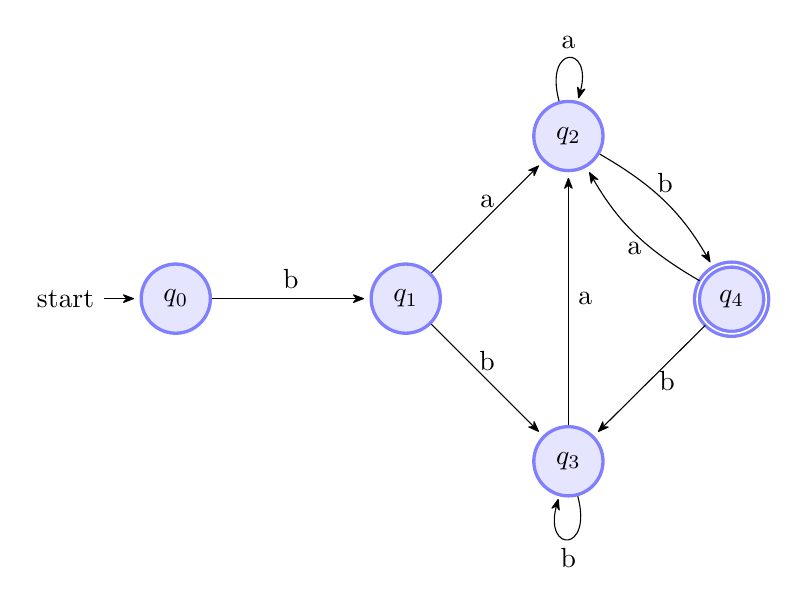
\begin{tikzpicture}[shorten >=2pt,
    node distance=2cm,
    % on grid,
    >={Stealth[round]},
    bend angle=15,
    every state/.style={draw=blue!50,very thick,fill=blue!10}]

    \node[state,initial]  (q_0)                      {$q_0$};

    \node[state]          (q_1) [right=of q_0] {$q_1$};
    \node[state]          (q_2) [above right=of q_1] {$q_2$};
    \node[state]          (q_3) [below right=of q_1] {$q_3$};
    \node[state,accepting](q_4) [below right=of q_2] {$q_4$};


    \path[->]
    (q_0) edge              node [above]  {b} (q_1)
    (q_1) edge              node [above]  {a} (q_2)
    (q_1) edge              node [above]  {b} (q_3)
    (q_2) edge [loop above] node [above]  {a} (q_2)
    (q_2) edge [bend left]  node [above]  {b} (q_4)
    (q_3) edge [loop below] node [below]  {b} (q_3)
    (q_3) edge              node [right]  {a} (q_2)
    (q_4) edge              node [right]  {b} (q_3)
    (q_4) edge  [bend left] node [below]  {a} (q_2)
    ;
\end{tikzpicture}\\

\subsection{将得到的DFA图的状态最小化\textcolor{red}{(15分)}}

$G_1$是接受状态的集合,$G_2$是非接受状态的集合,所以
$$
    G_1 = \{q_4\} ,G_2 = \{q_0,q_1,q_2,q_3\} \\
$$
$G_1$无法继续分割,故考察$G_2$
\begin{table}[h!]
    \begin{center}
        \begin{tabular}{c|c|c}
            \textbf{状态} & \textbf{a} & \textbf{b} \\
            \hline
            $q_0$       &            & $q_1$      \\
            $q_1$       & $q_2$      & $q_3$      \\
            $q_2$       & $q_2$      & $q_4$      \\
            $q_3$       & $q_2$      & $q_3$      \\
        \end{tabular}
        \caption{状态转换表(最小化)}
    \end{center}
\end{table}
可以看出,$G_2$中的状态$q_1$和$q_3$可以合并
故可以最小化DFA\\

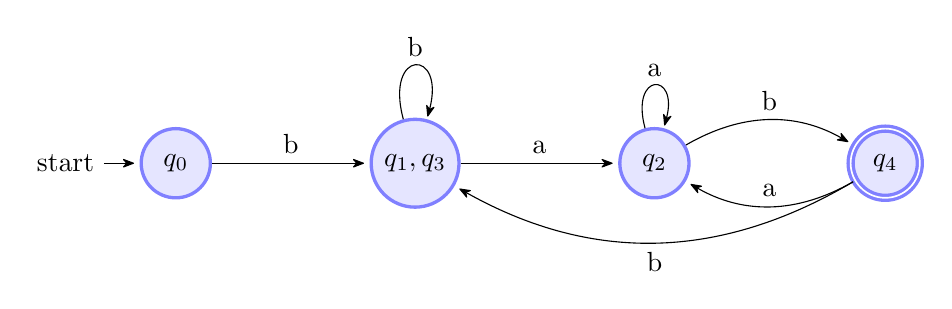
\begin{tikzpicture}[shorten >=2pt,
    node distance=2cm,
    % on grid,
    >={Stealth[round]},
    bend angle=30,
    every state/.style={draw=blue!50,very thick,fill=blue!10}]

    \node[state,initial]  (q_0)                      {$q_0$};

    \node[state]          (q_1) [right=of q_0] {$q_1,q_3$};
    \node[state]          (q_2) [right=of q_1] {$q_2$};
    \node[state,accepting](q_4) [right=of q_2] {$q_4$};


    \path[->]
    (q_0) edge              node [above]  {b} (q_1)
    (q_1) edge              node [above]  {a} (q_2)
    (q_1) edge [loop above] node [above]  {b} (q_1)
    (q_2) edge [bend left]  node [above]  {b} (q_4)
    (q_2) edge [loop above] node [above]  {a} (q_2)
    (q_4) edge [bend left]  node [above]  {a} (q_2)
    (q_4) edge [bend left]  node [below]  {b} (q_1)


    ;
\end{tikzpicture}
\section{给定文法}
\begin{equation*}
    \begin{aligned}
        S & \to {\rm if}\  E\  {\rm then}\  S \  {\rm else} \  S \\
        S & \to {\rm if}\  E\  {\rm then}\  S                    \\
        S & \to {\rm other}                                      \\
        E & \to b                                                \\
    \end{aligned}
\end{equation*}

\subsection{计算文法中非终结符的First集\textcolor{red}{(10分)}和Follow集\textcolor{red}{(10分)}}

提取左公因子,文法改写为

\begin{equation*}
    \begin{aligned}
        S  & \to {\rm if}\  E\  {\rm then}\  S \  S' \  | \  {\rm other} \\
        S' & \to {\rm else} \  S \  | \  \epsilon                        \\
        E  & \to b                                                       \\
    \end{aligned}
\end{equation*}
计算First集和Follow集
\begin{equation*}
    \begin{aligned}
        First(S)   & = \{{\rm if}, {\rm other}\} \\
        First(S')  & = \{{\rm else}, \epsilon \} \\
        First(E)   & = \{b\}                     \\
        Follow(S)  & = \{{\rm else}, \$ \}       \\
        Follow(S') & = \{{\rm else}, \$ \}       \\
        Follow(E)  & = \{ {\rm then} \}          \\
        % First(S') \cup Follow(S') & = \{{\rm else} \}           \\
    \end{aligned}
\end{equation*}
\subsection{构造它的预测分析表\textcolor{red}{(共20分,每空4分)}}

\begin{table}[ht]
    \begin{center}
        \begin{tabular}{c|c|c|c|c|c|c}
            \textbf{非终结符} & \textbf{if}                                & \textbf{then} & \textbf{else}          & \textbf{other}      & $b$      & $\$$            \\
            \hline
            $S$           & $S   \to {\rm if}\ E\ {\rm then}\ S \ S' $ &               &                        & $S\to\ {\rm other}$ &          &                 \\
            \hline
            $S'$          &                                            &               & $S'\to\epsilon $       &                     &          & $S'\to\epsilon$ \\
                          &                                            &               & $S' \to{\rm else}\ S'$ &                     &          &                 \\
            \hline
            $E$           &                                            &               &                        &                     & $E\to b$ &                 \\
        \end{tabular}
        \caption{预测分析表}
    \end{center}
\end{table}
\subsection{判断其是否为LL(1)文法\textcolor{red}{(共10分,理由5分,结论5分)}}

文法无左递归,但是
\begin{equation*}
    First(S') \cup Follow(S')  = \{{\rm else} \}
\end{equation*}
(或答:预测分析表中出现冲突)\\
所以文法不是LL(1)文法
\end{document}